\chapter{Context and problematic}

\section{Crisis Management}
\subsection{A definition?}
Defining the concept of crisis provides a hint of the challenges that lie within this domain.
Although the term is widely adopted in everyday language, it is paradoxically challenging to give a precise and definitive scientific definition.
The term is used every day for both financial crashes, natural or humanitarian disasters, or personal situations.
Many researchers have tried to define this vague concept.
\textcite{lagadecGESTIONCRISES1994} identified numerous attempts of definitions.
Among them, \textcite{rosenthalCrisisDecisionMakingNetherlands1986} proposed a taxonomy that would reflect the variety of types of crises:

\begin{itemize}
    \item The "unimaginable" crisis requires that we question the unthinkable.
    \item The "neglected" crisis is caused by a lack of interest or care.
    \item The "almost inevitable" crisis, despite preventive action.
    \item The "compulsive" crisis results from inadequate management.
    \item The crisis sought by some, internal or external, actors.
    \item The crisis deeply desired by all parties.
\end{itemize}

In an almost similar way, \textcite{mitroffStructureManmadeOrganizational1988} proposed a classification of crises according to intrinsic characteristics.
The authors use a 2D matrix to classify the different types of events.
One of the components opposes the origin of the event (internal or external), while the other axis opposes the "social" or "technical" aspects.
For instance, company bankruptcies are located in the internal/technical quadrant, terrorist attacks in the external/human quadrant, or natural disasters in the external/technical quadrant.
Brief definitions have also been proposed to define the term itself.
\textcite{hermannIssuesStudyInternational1972} proposed that "a crisis is a situation that threatens the essential goals of the decision-making units,
reduces the time available for decision-making, and whose occurrence surprises those in charge."
More than a simple situation, \textcite{rosenthalCrisisDecisionMakingNetherlands1986} will prefer to insist on the notion of crucial decision-making:
"A crisis is a serious threat affecting the basic structures or the fundamental values and norms of a social system, which—in a situation of high pressure and high uncertainty—requires crucial decisions to be made."
Nevertheless, crises are also periods of uncertainty and disarray of organizations, where rules and processes are blurred.
\textcite{lagadecGESTIONCRISES1994}, realizing the complexity of these phenomenons, abandoned the idea of a succinct definition.
Thus, he proposed a more ambitious, complete definition through a higher-level viewpoint:
\blockquote{A situation where multiple organizations, facing critical problems, subjected to strong external pressures, bitter internal tensions, are suddenly and for a long time projected on the front of the scene;
    all this in a society of mass communication, that is to say, 'live,' with the assurance of being on the front page of the radio news.}

From the definitions given above, one can see the difficulty of defining the concept of crisis, as it is so diverse.
This diversity in the use of the term reflects somewhat the very character of the crises.
By nature, crises are a constantly renewing phenomenon.
New causes, consequences, or ways to impact societies emerge.
This constant innovation might be what prevents any final definition.
In the end, crises seem to be the demons living in the dark face of our societies.
Invisible and seemingly out of reach, societies only witness their sudden and brutal irruptions in the tangible phase of our world.
These irruptions invariably result in an eruption of chaos.
This metaphorical representation translates a personal vision of what a crisis is and the inherent complexity of the definition of this concept.
However, while describing those "demons" seems a challenging endeavor, the irruptions themselves and their consequences possess common points.
The following part discusses these points.

\subsection{Characteristics of a crisis}
It now appears that a fixed definition of the concept of crisis is difficult to achieve.
However, if the concept of crisis remains vague, the effects and consequences are tangible and quantifiable.
Victims, material damages, environmental destructions, and other more or less reversible consequences are tangible.
A first characteristic extracted from the previous definitions is the emergence of chaos that creates a brutal rupture.
Crises are thus to be distinguished from incidents, which are difficulties for which preventive measures allow to keep the situation under control.
Without a definition, having an overview of the multi-dimensional consequences of crises is essential in building an adequate representation of the concept.
The literature is rich in numerous efforts to list the manifestations of crises.
Many authors, sharing the observation that it is difficult to define the phenomenon, even propose to define crises based on their consequences.
Thus, for \textcite{milburnManagementCrisis1972}, only an event that meets specific criteria would be eligible for the title of crisis.
The characteristics they evoke are:

\begin{itemize}
    \item Threat to assets identified as essential by managers.
    \item Need for quick decisions.
    \item Relatively short time frame for response.
    \item Lack of emergency measures available since it is an unforeseen situation.
    \item Need for innovation in solving the problem due to the absence of a pre-existing system.
    \item Information overload.
    \item Ambiguity.
    \item Increase in the number and importance of requirements.
    \item Internal conflicts in the organization.
    \item Considerable fatigue.
\end{itemize}

These first characteristics are discussed by \textcite{rosenthalCrisisDecisionMakingNetherlands1986}.
The latter propose characteristics that frame the effects of a crisis.
They consider that the previous characteristics do not sufficiently take into account all the facets of crisis.
In particular, the authors consider that crises are also times that create opportunities for certain individuals.
In a similar approach, \textcite{finkCrisisManagementPlanning1986} defines crises as situations that expose to risks.
The risks he identifies include:

\begin{itemize}
    \item Escalate;
    \item Attract significant media and administrative attention;
    \item Affect the regular operation of the company;
    \item Call into question the public image of the firm and its leaders;
    \item Reach the very foundations of the organization.
\end{itemize}

\textcite{lagadecGESTIONCRISES1994} summarizes the two previous authors through three main characteristics:

\begin{itemize}
    \item Surge: A crisis is a tsunami. Information, issues, external actors involved, media attention, etc.
          Regular processing capacities are overwhelmed as everything is tenfold.
    \item Disruption: The universe in which the organization/system was is falling apart. Allies are disengaging. New, unusual actors (and, most often, unwanted) appear.
          An overall ambiguity is cast onto the system hit.
    \item Breakdown: The system is falling apart. The regularity is not anymore. All reference points, both internal and external, are disappearing.
          All the decisions are "no-win" for the organization.
\end{itemize}

These characteristics adopt a high-level point of view and encapsulate many concepts.
They also provide valuable information to create a big picture of what a crisis is.
Differently, \textcite{fertierInterpretationAutomatiqueDonnees2018} proposed a set of four characteristics allowing to position crises relatively to each other:

\begin{itemize}
    \item Geographic scope of the event.
    \item Duration (time between the first and last consequences, including replicas).
    \item The \emph{severity} of the event (minor/major). Scale established according to the number of victims and or material damage.
    \item The \emph{complexity} of the event, depending on the number of dimensions involved in the event, the number of layers and replicas of the crisis.
\end{itemize}

These criteria can be used as metrics to compare different events according to the impact they had.
Also, it highlights how crisis events are composed of a wide diversity of consequences.
Characterizing such events benefits from a multidisciplinary approach, as different viewpoints lead to a different picture of the crisis phenomenon.
The following paragraph presents the different terms used in this manuscript and provides the semantics associated with them.

\subsection{Schematic representation of the components of crisis}
% TODO Figure pour illustrer les différents termes (page entière probablement)
During nominal times, the \emph{population} lives in an \emph{environment} in which existing \emph{systems} are composed of valuable \emph{assets} managed by \emph{organizations}.
Usually, when one studies a crisis, the point of view of an organization is taken.
The environment refers here to everything that is outside of the system or organization of interest.
The immediate environment can be composed of other assets part of other systems or organizations.
It can be other companies, other cities, other countries, etc.
In the environment, there are systems and their associated organizations that are impacted.
The part of the population that suffers from the event is considered as the \emph{victims} of the event.
Among all these systems, there is one of particular interest when a crisis happens: the crisis management system, which is in charge of the response to the event.
At crisis time, the organization in charge of crisis management creates a \emph{crisis cell}.
The United Nations Department of Humanitarian Affairs \parencite{undepartmentofhumanitarianaffairsInternationallyAgreedGlossary1992} defines a crisis cell as:
\blockquote{A facility officially designated for the direction and coordination of all actions in the response phase of a crisis.}
The crisis cell is composed of \emph{operators} that gather, filter and share incoming information with the \emph{decision-makers}.
The latter make \emph{decisions}, some of which are instructions to the \emph{response teams}.
The framework proposed is thus composed of four main entities: the environment, the system, the organization, and the decision-makers.
The following sections describe each of the entities proposed.

\subsubsection{The environment}
The environment represents an area.
This entity is linked to the geographical characteristic proposed by \textcite{fertierInterpretationAutomatiqueDonnees2018}.
When an event occurs, the environment can be split into two parts: a part impacted by the event (the crisis environment) and a part not impacted.
Some events can concern only a small industrial area, as in the case of water pollution, for instance, or have a worldwide scale, as in the case of the global pandemic that the world is facing at the time of writing this document.
Events with different scales involve actors accordingly.
A crisis can affect the environment in which systems and organizations exist in several ways.
Part of what defines a crisis is this sudden change in the environment.
Decision-makers find themselves disoriented.
Infrastructures, resources, or actors that were supposed to be available are not anymore, or their status is unknown to the decision-makers.
Crises reshape the environment, and consequently, the first step is taken once the organization realizes that they lost control of the situation is to figure out what this new environment is.
However, not only the environment of the system is reshaping, but the system itself is too.

\subsubsection{The system}
A system is a set of organizations that rely on resources that compose their stakes.
In this definition, a city is a system composed of many organizations.
The latter use different resources to function.
A crisis affects a system if and only if the system's stakes are threatened.
For instance, a volcanic eruption in the middle of a desert will probably not be considered a crisis event.
On the other hand, a volcanic eruption near a city is a disaster event.
The former would be a dramatic event, while the latter would probably modify a few air traffic lanes.
Crises often result from a combination of different factors.
The organization in charge of the systems is supposed to protect the known vulnerabilities of the system and prepare for the unknown ones.
A crisis can emerge from a stressful event on one of those vulnerabilities.
To illustrate those interactions, \textcite{benabenCollaborativeSystemsCrisis2014} propose a framework that illustrates the relationship between the different concepts Figure~\ref{context:fred-framework}.
According to the previous authors, the consequences are the result of an event on risks (which we call here vulnerabilities).
These risks are, in turn, the result of dangers on stakes.

\begin{figure}[htb]
    \centering
    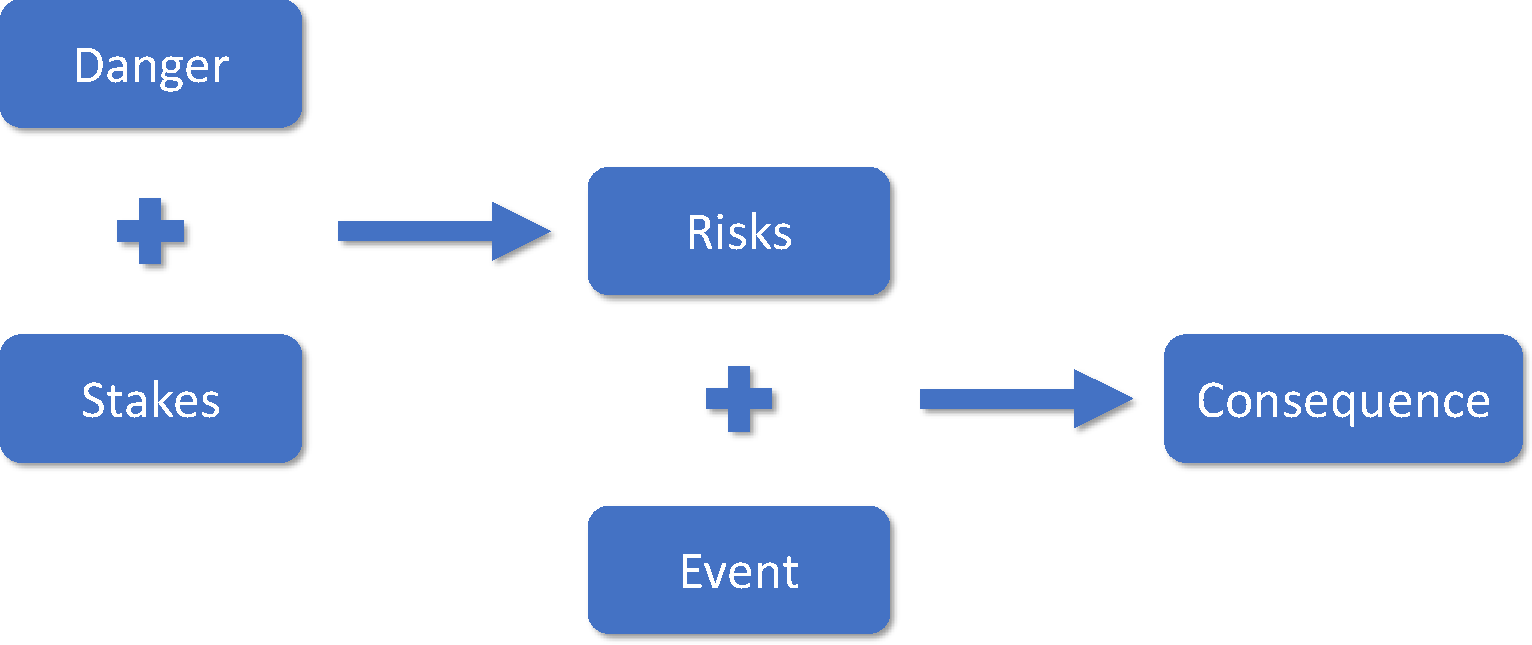
\includegraphics[width=\textwidth]{figures/chap-1/fred-consequences-framework.pdf}
    \caption{Crisis causality chain from \textcite{benabenCollaborativeSystemsCrisis2014}}
    \label{context:fred-framework}
\end{figure}
\label{sec:danger-risk-consequence}

Each consequence can, in turn, become a danger or an event that endangers the system.
This phenomenon is referred to as the "cascading effect."
The crisis is self-feeding, with the dynamism explained before, and drags the system in its fall.
The best known industrial example is undoubtedly the Chernobyl nuclear disaster.
The cascading effect also joins the "surge" evoked by \textcite{lagadecGESTIONCRISES1994}, which is based on numerous testimonies of people who were involved in the crisis management.
In the end, a complete disruption of the system occurs.
Regular operation is no longer possible.
Existing processes are no longer valid.
The historical partners are no longer available while unusual actors appear.
One of the consequences of this disruption is the increasing complexity of conducting operations.
Additional precautions are required for each decision and intervention that follows.
Every action that was once trivial becomes uncertain.
Most of the usual signals have disappeared, and the remaining ones are ambiguous.
At the same time, the information requirements for each decision explode.
The parts of the system that the event has not destroyed are then rendered inoperative.

\subsubsection{The organization}
An organization is a group of individuals that compose and manage a part of the system.
Companies, public services, NGOs, crisis management teams are considered as organizations.
This definition is recursive: an organization can be considered as a system.
Thus, the organization's services become the different organizations that compose the system.
Each organization has to respond to the event that hit its system.
They activate their services dedicated to crisis response.
During response time, each organization attempt to protect their stakes and their resources.

The activation of the response depends on how long it takes the organization to realize that the event is there.
There may be a lag time between the first effect of the crisis and the activation of the response.
By the time the response is activated, the crisis has already impacted a significant part of the system.
From that moment, the state of the system is altered.
This change plunges the organization into uncertainty and doubt.
The system is no longer in a known state.
The situational awareness has changed, and there is an urgent need to re-establish a coherent vision for further response operations.
The importance of situational awareness is further developed in the second chapter.
From that moment on, the organization will seek to obtain as much information as possible about its environment and its system.
Each decision becomes crucial in the protection of the stakes.
However, with the loss of knowledge about the system's state, every decision comes with much uncertainty.

To reduce uncertainty, the organization will seek to know the state of the system.
It, therefore, requires reports on all aspects of the system.
Information from automated parts of the system might be automatically retrieved if they are equipped with the appropriate sensors.
Emergency services, such as the American 911, firefighters services, etc., obtain mainly their information from the response teams deployed and victims' calls.
Similarly, external services (meteorological, specialists, etc.) can also provide external data to help the organization make decisions.
However, the organization is rarely prepared to handle such a volume of information
As a result, the decision-makers at the head of the organization become overwhelmed.

In addition to this, the initial information feedback is scattered and therefore ambiguous.
The context in which each piece of information fits is absent or limited.
The situation faced by the organization can be illustrated with a puzzle.
However, we do not know the outcome of the puzzle, and the pieces are provided to us one after the other, in no particular order.
We are also forced to place the puzzle pieces (i.e., make decisions) without knowing what the following pieces will be.
Under these conditions, it is only possible to complete the puzzle when enough pieces are provided.
To imagine the psychological consequences of such a way of completing the puzzle makes it obvious why we do not do puzzles in this way.

In addition to these internal difficulties, there is also external pressure.
The event inevitably attracts the attention of regulators, higher authorities, and the media.
The organization, sometimes unknown until then, finds itself under the spotlight.
Its past is scrutinized, looking for previous mistakes that may have led (or not) to the current event.
Its leaders and their decisions are dissected, and the inconsistencies are highlighted as soon as possible to feed the headlines.
Damages caused to the organization are not limited to physical ones.
Its image and reputation might also be impacted, especially if the management is not
Thus, in addition to the physical impact of the crisis, the trust and the image of the organization are also weakened.

\subsubsection{The decision-makers}
The decision-makers are the people with responsibility in the organization.
As most organizations are hierarchical, they have layers of decision-makers, each responsible for an area of the organization.
Decisions made by some individuals thus take precedence over those made by their subordinates.
During an ongoing event, this phenomenon might impede action.

Moreover, most of the decisions appear as "no-win" for the organization.
Problems accumulate without time to solve any for fear of making the situation worse.
The decision-makers, once in control of the situation, are getting paralyzed.
With the knowledge of their environment gone, they find themselves stuck.
Their perception is distorted, as much as their assumptions.
They soon realize that the situation is incredibly complex, and yet they have to move on.
All this is done in a hurry, created by the influx of requests and reports.
Decision-making is further complicated because the usual processes and safeguards they used to rely on potentially no longer exist or have become irrelevant.
Once feared, improvisation and innovation are now required to realize that inaction will be as, if not more, costly than action.
The stress on the organization is hitting decision-makers hard.
Under the urgency, stress, and fatigue, every decision becomes a battle to be fought in the war created by the crisis.

This first part of the chapter presents a personal vision of crises and what they imply.
This vision will drive the manuscript, including the structure of the different concepts affected by a crisis - the environment, the system, the organization, and the decision-makers.
The remainder of this section develops how organizations deal with these situations.

\subsection{Crisis Management}
Crises are not a question of "if" but of "when."
This inevitability implies an upstream reflection on the part of organizations and a consideration of this problem within the systems.
These practices are called \emph{crisis management}.
Crisis management is
\blockquote{The set of organizational modes, techniques, and means that allow an organization to prevent,
    prepare for and respond with the occurrence of a crisis, and then draw lessons from the event to improve procedures and structures
    with a forward-looking vision (Wikipedia, 2021).}
This definition perfectly highlights two main characteristics of crisis management.
First, crisis management is more a broad spectrum methodological toolbox than a set of recipes to be applied in an event.
Secondly, it takes into account the different temporal phases of the crisis.
In the following, we detail these two aspects.

\subsubsection{The Crisis Management cycle}
The crisis management literature identifies four major phases.
These phases are most often represented in the form of a cycle.
The 4 phases are :

\begin{itemize}
    \item Prevention: phase aiming at preventing the appearance or reducing the effect of an emergency.
          This phase consists of identifying potential hazards that threaten system vulnerabilities and appropriate measures.
    \item Preparedness: measures that facilitate the response to the disaster. It involves ensuring that resources are available and deployable, that response personnel are trained, and that the potentially impacted organization is psychologically prepared.
    \item Response: corresponds to the activation of the measures prepared previously.
    \item Recovery: the phase that follows the response to the crisis. It corresponds to the repair/reconstruction of the parts of the system impacted by the event.
          This stage is often accompanied by an analysis of the risks associated with the repairs to avoid creating a replica of the crisis.
\end{itemize}

In this cycle, only one transition between two phases is clear: the one between preparation and response.
This transition occurs when the organization acknowledges the event and goes into crisis management.
The other transitions correspond more to a period where two phases coexist.
The prevention phase, however, leads to some debate.
\textcite{benabenCollaborativeSystemsCrisis2014} argue that the prevention phase is, in fact, common to the whole cycle.
Even during the response and the recovery, the organization observes prevention measures to prevent cascading effects.
Therefore, prevention can be considered as constant.
The crisis management cycle can be simplified with only three phases in crisis management: the preparation (before the event), the response (during the event), the recovery (after the event).

Also, it is possible to see beyond the cyclic representation.
Today's world is complex, tense, and deeply interconnected \parencite{benabenInstabilityNormPhysicsbased2021}.
As a result, large organizations or countries possess a large surface vulnerable to potentially disruptive events.
Then, instability and crisis management somehow become the norm.
Small and large events trigger responses from the organization.
However, these events are concurrent, and each one is at a specific phase of the cycle.
Consequently, looking at the global picture, these organizations are dealing with multiple crises simultaneously.
Similarly, significant crises are often not dealt with at the global level directly.
For instance, a local firefighters station will not deal with a whole hurricane by itself.
Instead, it will take care of smaller, local events that are the direct consequences of the hurricane.
In this example, the hurricane triggers the response phase in the cycle, but one could zoom into the "response phase" of the cycle.
Each consequence of the hurricane can be imagined as a local crisis, each triggering its own cycles.
As a result, there is a macro event (the hurricane) and several smaller and concurrent cycles happening simultaneously.
The cycle representation of crisis management does not account for the scale or the complexity of events.
It is, however, a good enough abstraction to represent the different times in an event.

\subsubsection{Stakes in Crisis Management}
Crisis management techniques are the set of tools used to respond to crises.
They are used by crisis management organizations at the onset of an event.
This organization faces various challenges in its mission to respond to the event.
\textcite[12--18]{fertierInterpretationAutomatiqueDonnees2018} identifies five challenges for the organization:

\begin{itemize}
    \item Collaborate with internal and external stakeholders.
    \item Recover a situational awareness of the environment and the system (see section \hyperref[sec:situational-awareness]{3.2.1}).
    \item Manage data collection from multiple sources.
    \item Process the previous data to get relevant information.
    \item Have and maintain a system to automate the previous two points.
\end{itemize}

\textcite{batardIntegrerContributionsCitoyennes2021} also identifies two of the previous challenges as the top ones in crisis response: i) having sufficient situational awareness, and ii) coordinate the different actors of the response.
From these two main stakes, the author then proposes four axes to protect those.

First, managing the multiplicity of data sources.
Organizations in charge of crisis management are already used to taking into account several data sources.
Feedback from the field from the staff allocated to the response and phone calls from victims or witnesses of the event are commonly used.
However, new sources are emerging.
The Internet of Things and the variety of sensors that compose it can provide records of interests.
The rapid and global development of social media is also a potentially attractive source of data \parencite{meierStrengtheningHumanitarianInformation2013}.
The opportunities offered by this data source are detailed in section \hyperref[sec:nlp]{1.2.3}.

Secondly, automatically interpret these data to extract relevant information.
This information should then be delivered in an adapted way to the decision-makers \parencite{luokkalaDevelopingInformationSystems2014,vandewalleImprovingSituationAwareness2016}.

Thirdly, the management of information systems adapted to the crisis management context.
This information system is supported by an IT system whose role is to facilitate the response.
This facilitation is enabled by delegating some of the tasks necessary to i) restore situational awareness and ii) coordinate actors to the IT system \parencite{benabenManagementCollaborativeBehavior2015}.

Fourth, the information system and the computer system must be adaptable.
This strong constraint results from the nature of crises.
A crisis management system must therefore be able to detect changes in the situation and react to them in an adapted manner \parencite{barthe-delanoeEventdrivenAgilityInteroperability2014,charlesModelDefineAssess2010}.

The two previous analyses highlight primary challenges during crisis management.

\begin{enumerate}
    \item Understanding the current situation and state of the environment.
    \item Coordinate the response of actors fluidly, following their skills and needs.
    \item Automatically collects and organizes available data.
    \item Automatically manages the information obtained and distributes it efficiently to decision-makers.
\end{enumerate}

Thus, the organization responsible for crisis management must first restore its knowledge using its available data.
Secondly, it must manage the information obtained from these data to best coordinate its response with its internal and external actors.

\subsection{Tools for Crisis Management}
The previous section identified two major stakes from the information system point of view: the coordination of the actors and the restoration, than management of the situational awareness.
The protection of these stakes by the system is of the utmost importance to allow an adequate response.
Tools and practices have been developed to help organizations in charge of crisis response to address those issues.

\subsubsection{Organizational modes}
The organization of the response is one of the components of the preparation phase.
During this phase, the different future actors of crisis response agree on the roles and responsibilities during the future event.
For instance, in the response phase, the system dealing with the response uses a hierarchical organization layered with crisis cells.
A crisis cell is a facility officially designated for the direction and coordination of all actions in the response phase of a crisis.
They bring together the organization's decision-makers who implement and direct the various actors to respond to the crisis.
Thus, the crisis units must have a high-level vision of the event and be close to the actors of the response they are managing.
Large-scale crises (mobilizing many actors or a large territory, for example) will undoubtedly create a hierarchy of crisis units.
While the "low-level" crisis units orchestrate the response, a "higher-level" crisis unit is responsible for transmitting information between the "low-level" crisis units and coordinating their responses.
In France, this hierarchy and the role of each actor are described in the ORSEC plan~\footnote{https://www.gouvernement.fr/risques/dispositif-orsec}.
The hierarchy itself is composed of 5 levels:

\begin{itemize}
    \item European
    \item National
    \item Zonal
    \item Departemental
    \item County
\end{itemize}

Each of the crisis cells set up has its specificities, depending on the actors who compose it.
However, all are constrained by the same need for collaboration \parencite{benabenAIFrameworkMetamodel2020,comfortCrisisManagementHindsight2007} and information \parencite{comfortCrisisManagementHindsight2007,endsleyTheorySituationAwareness1995}.
It is precisely the role of the information system to manage and exchange situation-specific information between the different actors.

\subsubsection{Techniques and Methods}
The organization mentioned above is only effective if the actors coordinate their actions.
This coordination requires the communication of information available to the different actors.
The organization's information system is in charge of this aspect.

This dissertation uses the following definition of information systems.
\blockquote{An information system (IS) is a formal, sociotechnical, organizational system designed to collect, process, store, and distribute information.
    From a sociotechnical perspective, information systems are composed of four components: task, people, structure (or roles), and technology.
    Information systems can be defined as an integration of components for collection, storage, and processing of data of which the data is used
    to provide information, contribute to knowledge as well as digital products that facilitate decision-making \parencite{InformationSystem2021}.}
This definition mixes the definition provided by \parencite{oharaManagingThreeLevels1999,piccoliInformationSystemsManagers2019,zwassInformationSystemDefinition}.
Thus, the organization's information system is the cornerstone of information management within the organization.
It can be digitalized or not, depending on the needs and practices of the organization, as it reflects how the information is processed in the physical organization.
The information system is an abstract concept that encompasses many aspects of the organization.
The development and maintenance of the information system are performed during the preparation phase.
During this phase, hardware and software must be deployed, tested, and used for training to ensure smooth operation during the response.
The hardware aspects are outside the scope of this manuscript, which is mainly interested in the software and social part of the information system Figure~\ref{context:information-system}.

\begin{figure}[htb]
    \centering
    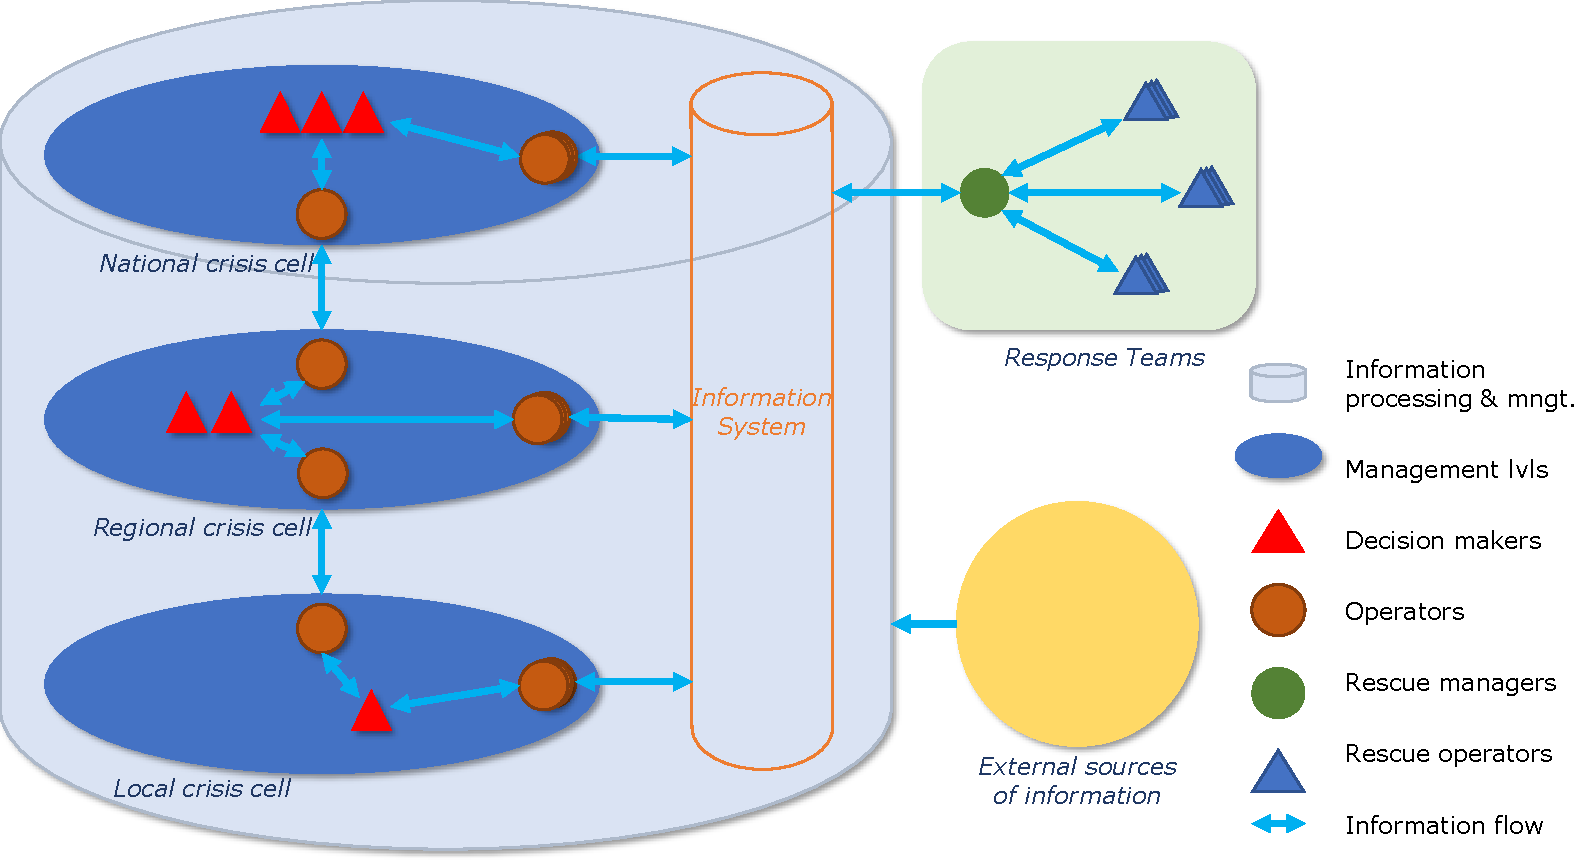
\includegraphics[width=\textwidth]{figures/chap-1/information-system.pdf}
    \caption{Representation of a crisis information systems and its interaction with the different members of the organization}
    \label{context:information-system}
\end{figure}

The role of an information system is, according to the definition, to collect, process, store and distribute information.
The information systems then allow their users to enter information into the system.
This information is then consumed through interfaces.
The information is automatically stored and processed by the system.
In France, \textcite{morelEtudePriseDecision2010} indicate that fire department services mainly receive their information from three sources:

\begin{itemize}
    \item Victims' calls made from emergency numbers.
    \item The crews deployed to respond to the crisis.
    \item Other organizations involved in crisis management.
\end{itemize}

One thing all this information has in common is that none of it is first-hand.
Moreover, how this information is collected is not necessarily representative of the situation experienced by the population.
These collection methods result in a relatively small volume of information compared to the number of people affected.
The information, therefore, does not systematically reflect the emergency experienced by the population.

The last part detailed the way crisis cells are organized in crisis response and the hierarchy built to scale decision-making with the size of the event.
Each actor of this hierarchy comes with its own internal information system.
However, to enable the coordination between all the different actors, information has to flow between each of them.
Nevertheless, two challenges arise.
First, the actors have to share a common vocabulary in order to communicate.
Secondly, the information system has to be designed to allow communication.

Misunderstandings between the different actors often hamper the distribution of information.
The latter often have different skills, responsibilities, and roles.
Therefore, each actor builds his own vocabulary and terminology to designate his field of action elements.
If this facilitates daily operations during an event, it complicates the collaboration and communication between the actors \textcite{opachMapbasedInterfacesCommon2020}.
Therefore, the preparation phase is an opportunity to identify the actors who will potentially be brought to collaborate during an event and bring them together to be familiar with each other's culture.

Standard format and representations of the information between all the actors are needed to build a shared understanding of the situation.
From a technical point of view, the different actors can decide to set up a "Common Operational Picture (COP)."
The U.S. Department of Homeland Security defined a COP as \parencite{u.s.departmentofhomelandsecurityNationalIncidentManagement2014}:
\blockquote{A representation that is established and maintained by collecting, collating, synthesizing, and disseminating information among the different participants.
    It allows the different actors to have access to the same information regarding the availability and location of resources and the status of different requests for assistance.}
This representation is often cartographic, allowing the geographic component of information to be easily represented.
Geographic information is also information that is equivocal among all actors.
The COP is, therefore, a tool that allows to initiate and build a dialogue between the different actors of the response.
It is also the visible face of the information system.
The COP benefits from all the advantages that the rest of the information system provides.
The COP can be automatically fed with the data mentioned above.
Thanks to this data, the information system can then produce helpful information for the decision-makers and automatically make it available on the COP \textcite{fertierInterpretationAutomatiqueDonnees2018}.
One of the problems currently faced by COPs is their inability to communicate with each other most of the time due to mutually exclusive software, which does not offer the possibility of dialogues between them \textcite{opachMapbasedInterfacesCommon2020}.

\begin{figure}[htb]
    \centering
    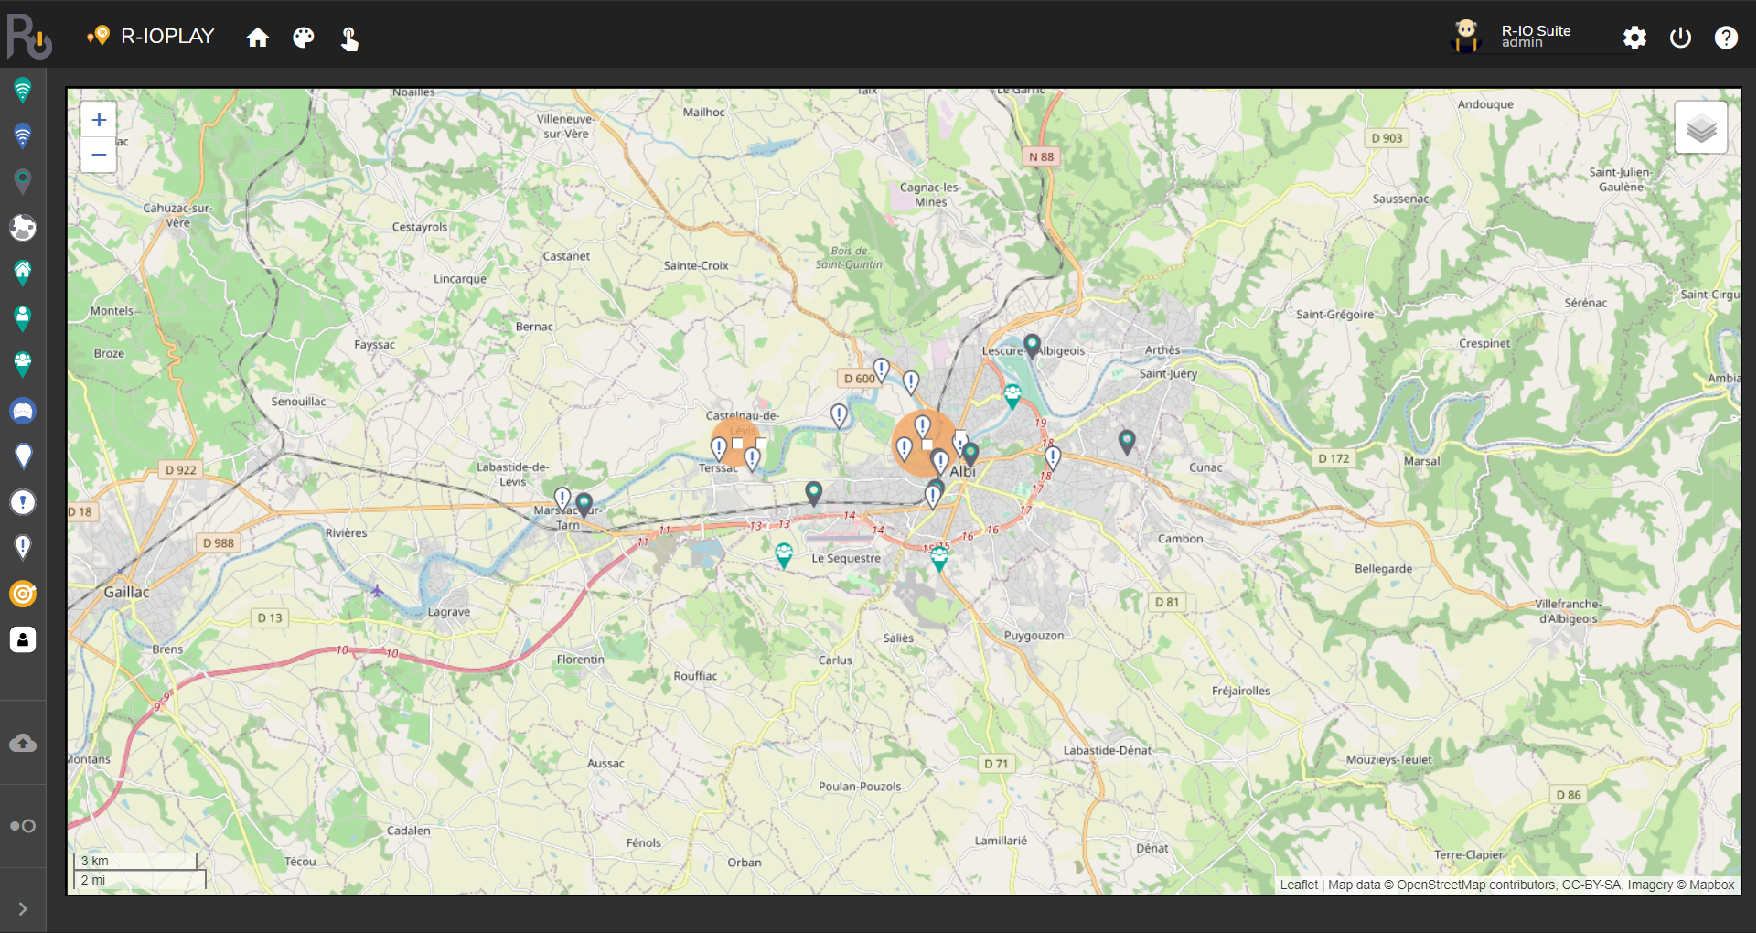
\includegraphics[width=\textwidth]{figures/chap-1/rio.pdf}
    \caption{Cartographic display of the R-IOSuite software in a flood scenario in France\protect\footnotemark}
    \label{context:cop}
\end{figure}
\footnotetext{https://research-gi.mines-albi.fr/display/RIOSUITE/Welcome}

Finally, the COP is an asset for building and maintaining adequate and shared situational awareness among all actors.
As we saw earlier, the restitution of situational awareness is one of the challenges of crisis management, as is the coordination between the different actors.
The COP is an asset because it is a tool that allows both issues to be addressed simultaneously.

Crisis management is a challenging domain.
By nature, crises events are uncertain and hard to define.
Nevertheless, patterns emerged from this uncertainty, especially when it comes to information management.
Regardless of the event, decision-makers are in dire need of information about the event's impact on their system and organization.
Tools and methodologies have then been developed to assist the decision-makers from the different organizations in coordinating and understanding the situation.
Research and development around digital tools to support information management occur in the crisis informatics domain \parencite{palenCrisisInformaticsHumancentered2020}.
One of those tools is the Common Operational Picture.
The COP is a map shared between the different actors, with standard but also specific information displayed.
This visual representation aims to be the interface between shared information systems used by the different actors.
However, the COP comes with its own challenge, as each information system has to share information with the common one.
Also, the different actors have to agree on common representations and terminologies used.

\section{Social Media}
\subsection{What are Social Media?}
The previous section highlighted the challenges faced in decision-making during crisis events.
At the same time, and somewhat paradoxically, our societies have never had that many ways and platforms to exchange information.
Among these platforms, social media have recently appeared.
Social media are Internet platforms that appeared during the Web 2.0 era.
The term Web 2.0 was developed between 2003 and 2007 by T. O'Reilly.
This terminology was initially born to revive the Web economy after the explosion of the dot com bubble formed during the development of Web 1.0, consisting mainly of web portals.
Web 2.0 reflects the development of the community web and is organized around platforms that allow their users to connect in order to co-create and share content \textcite{oreillyWhatWebDesign2007b}.
Social media fits into this definition.
\textcite{kaplanUsersWorldUnite2010} identify six types of social media: \emph{blogs and micro-blogs} (e.g., Twitter), \emph{social networking sites} (e.g., Facebook), \emph{collaborative projects} (e.g., Wikipedia), \emph{content communities} (e.g., Youtube), \emph{virtual social worlds} (e.g., Second Life) and \emph{virtual game worlds} (e.g., World of Warcraft).
Social media are now essential websites and platforms that have up to one billion users, in the case of Facebook.
Like the crises we mentioned earlier, it is difficult to grasp their full dimensions.
These platforms, often global, connect users worldwide, forming a digital twin of our societies.
The multitude of cultures, communities, languages, and codes that coexist in a single place has no equivalent in the history of humanity.
Opportunities and threats accompany the disproportionate size of these platforms.
Social media are indeed an excellent gateway to the world, allowing us to connect with an incredible number of people around the globe.
It is also an efficient way to share information and exchange with other users through many formats.
If the majority of social media users are consumers of content, a significant portion of them also creates content \parencite{fuchsSocialMediaCritical2021}.
Content creation on these platforms is thus their cornerstone, so much so that some of these platforms do not hesitate to pay their users who contribute, thus making a new profession emerge: content creator.

However, with this opportunity to unite humanity in a few hubs on the Internet comes many challenges.
False information spreading, harassment campaigns or state disinformation are some of the problems associated with social media.
If all these problems are not exclusive to these platforms, their dimensions and dynamics amplify them greatly.
The following sections emphasizes two components of social media: \emph{social network} and \emph{viral information}.

\subsection{Social Media characteristics}
\subsubsection{Social Network}
Most people live in a community.
Family, friends, neighbors, colleagues, all of these circles form an individual's social network.
The social network is an integral part of one's life.
Some researchers have looked into the question of what the social network of different individuals could be.

The mathematician \citeauthor{erdosEvolutionRandomGraphs1960}, while studying random networks, discovered that each node of the network is on average separated from any other node by six intermediate nodes \parencite{erdosEvolutionRandomGraphs1960}.
More surprisingly, this result is little affected by the size of the network.
A few years later, these theoretical results found a concrete application in social sciences.
\textcite{milgramSmallWorldProblem1967} verified the validity of the previous results within a population of individuals.
By measuring the number of intermediaries required to send a letter to a targeted person, \citeauthor{milgramSmallWorldProblem1967} validated \citeauthor{erdosEvolutionRandomGraphs1960} results.
In this experiment, each individual corresponds to a node in the network, and the edges are the relationships between the different individuals.
Their results obtained in this physical experiment validated the theoretical results on random networks.
This property is now known as the "six degrees of freedom" and refers to the average number of connexions required to link all nodes of the network.

\textcite{wattsCollectiveDynamicsSmallworld1998} sought to deepen the understanding of the six degrees of freedom and discovered on this occasion the structure in small worlds of social networks.
So if people meet each other by chance, as in Paul Erdös' model, the social network itself is instead composed of small communities, with many links between individuals
and very few links between communities.
This model is called a "small-world network" as most individuals are connected by very few intermediaries, regardless of the distance between them or the community to which they belong.

Similarly, \textcite{barabasiEmergenceScalingRandom1999} deepen Paul Erdös' random model by discovering another property of social networks.
Indeed, the random model predicts that the distribution of the number of friends among individuals must follow, by construction, a normal distribution.
However, this is not what they discover experimentally.
The distribution of the number of friends among individuals follows a power law.
This property thus forms a scale-invariant network, where individuals connect preferentially to the most influential nodes.

In reality, both models have their properties verified.
We can therefore consider, as a first approximation, that the two models coexist.
Therefore, a social network can be modeled through three main properties:

\begin{itemize}
    \item Each individual can be linked with any other, using only a few intermediaries (six on average), whatever the size of the network
    \item The network is structured in communities that are very connected to each other.
    \item The communities are connected by a few individuals who act as hubs.
\end{itemize}

These properties are illustrated in Figure~\ref{context:social-network}.

\begin{figure}[htb]
    \centering
    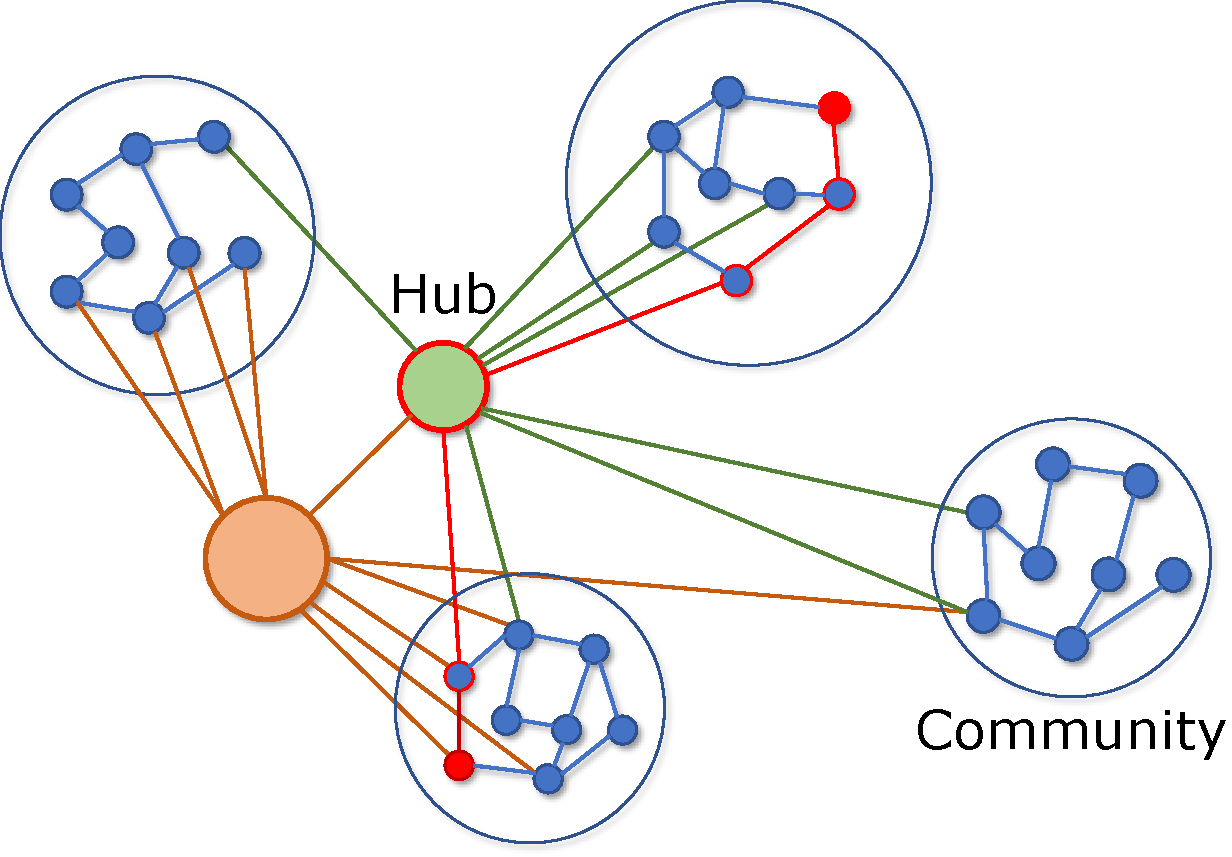
\includegraphics[width=\textwidth]{figures/chap-1/network.pdf}
    \caption{Illustration of the combination of both social network models from \textcite{wattsCollectiveDynamicsSmallworld1998} and \textcite{barabasiEmergenceScalingRandom1999}. The red path illustrates how two members of different communities can still be linked through few intermediaries.}
    \label{context:social-network}
\end{figure}

These properties are valid whether the social network is "real" or virtual - many of the experiments in the previous publications were obtained by studying social media.
Thus, social media can be seen as many communities linked together by hubs (influencers).
Having the structure of social networks in mind allows us better to understand the propagation of information within a social network.
This brings us to the following section and a topic familiar to all social media users: viral information.

\subsubsection{Virality}
The propagation of information, true or false, within a community is experienced daily by everyone.
However, this characteristic of information sharing is exacerbated in the case of social media for two reasons.
First, social media brings together a vast number of users in one place.
Second, they provide their users with several tools that aim to make information sharing much more straightforward.
By construction, social media put information and content sharing at the center of their strategy.
However, in a social network, each user can easily reach any user in very few intermediaries, regardless of the size of the network.
Moreover, information can quickly reach many users if it is shared through network hubs.

This speed of dissemination is thus unusual, as are the results that such propagation can generate.
Research teams are therefore interested in understanding what viral information is and how this virality is characterized.
By studying chains of information propagation, they identify that the phenomenon of virality is quite rare.
Large content cascades are the exception, not the rule.
99\% of posts are reposted less than ten times, while 0.001\% of the posts create cascades of more than 1,000 reposts.
Viral content is therefore rare, but it is seen by many users when it goes.

Recently, the notion of virality on social media has been widely associated with the term "fake news."
Fake news is a concern that grew with social media platforms themselves.
Notably, in the 2016 U.S. election context, the involvement of Russia in the process through disinformation campaigns \parencite{u.s.senateExtremistContentRussian2017}.
brought even more attention to that problem.
\textcite{lazerScienceFakeNews2018} define fake news as "fabricated information that mimics news media content in form but not in organizational process or intent."
The authors warn about the stakes and threats posed by fake news on our societies and call for more efforts to understand these dynamics, which are still largely misunderstood.
% TODO Explain why the next sentence in more details
Also, viral content cascades depend on the veracity of the content they propagate.
Thus, to more people, false information spreads faster for longer with an essentially vertical structure (friends of friends relay the information).
On the contrary, accurate information spreads more slowly, to fewer people, with slower kinetics and an essentially horizontal structure (the sender's followers essentially share the information).
Deriving from the previous results, \textcite{vosoughiRumorGaugePredicting2017} built a system that assesses the veracity of one piece of information based on the way this information is propagated.

Finally, the understanding of the propagation of information on social media remains largely marginal.
The call to link more independent research to the platforms of \textcite{lazerScienceFakeNews2018} remains anecdotal mainly, effectively hindering progress in this field.
In the following section, we explore the different opportunities for crisis management in light of the few elements presented so far on social media.

\subsection{Opportunities and Threats posed by Social Media for Crisis Management}
The previous sections highlight how social media were similar to a digital twin of society.
These platforms offer a point of view never seen before.

Significant events have long had an imprint on the Internet.
In the aftermath of the September 11 attacks in New York, web pages for exchanging information about people were created \parencite{palenCitizenCommunicationsCrisis2007}.
The relationship between crisis events and social media is now well established.
The case of the ditching of the U.S. Airways Flight 1549 on the Hudson River in New York City in January 2009 is often used as an example of the impact that social media can have in essential situations.
The information of the ditching had indeed been relayed on social media before all the traditional media \parencite{murthyTwitter2018}.
Other studies have highlighted the reaction of social media during crises, as in the case of tornadoes in the United States \parencite{justinei.blanfordTweetingTornadoes2014}.

However, crisis management requires data and information to be able to achieve its objectives.
Social media appear as a potential source of information for emergency services \parencite{tapiaSeekingTrustworthyTweet2011}.
Moreover, where phone calls were the only link with the population, this digital twin of society offers a real-time overview of the conversations and feelings of the people who are affected by the event.
These platforms thus make available a wide variety of data, which can help emergency services.
As content creation platforms, users can use the wide range of tools at their disposal to share information about the ongoing event.
Texts, photos, and videos can help crisis decision-makers better understand the event, even in places with no resources deployed.
Social media can also bring back information that other actors within the organization may have missed.
Finally, users of these platforms not directly impacted may decide to help the victims.
These volunteers, digital or not, could be mobilized to assist the emergency teams deployed on the scene of the event \parencite{batardIntegrerContributionsCitoyennes2021}.

The full potential of social media is yet to be discovered.
However, these platforms come with challenges.
As mentioned in the previous section, fake news is a current problem with social media \parencite{lazerScienceFakeNews2018,vosoughiSpreadTrueFalse2018,oshikawaSurveyNaturalLanguage2018}.
This phenomenon is also mentioned in crisis management and attracts some interest from the scientific community \parencite{starbirdExaminingAlternativeMedia2017,sellMisinformationUSEbola2020}.
However, while misinformation and the sharing of false information we see on social media in crises, it is not necessarily indicative of their uses alone.
\textcite{bubendorffConstructionDisseminationInformation2021} present the small amount of information involved and the self-correcting effect of the crowd, which ultimately reduces the impact of false information.
Despite this, emergency services remain cautious about the use of information from social media.
\textcite{tapiaGoodEnoughGood2014} investigate their fears and what motivates this behavior.
In particular, the previous authors highlight that social media do not necessarily provide more misleading information than phone calls.
Their fears stem mainly from the relative novelty of social media and the lack of understanding of their universe.

Social media are Internet platforms that provide content creation tools to their users, generating and sharing data.
Altogether, Twitter, Facebook, Reddit, Instagram, Youtube, and many others, have billions of users worldwide who share their everyday life, creations, and feelings with their communities.
These digital twins of the society are resourceful and possess valuable information for crisis management.
However, the dynamic of these platforms remains hard to understand for individuals.
Also, in light of the recent controversies that have sprung, many are questioning their utility to ease crisis response.
Social media provide a vast amount of

\section{Natural Language Processing}
\label{sec:nlp}
\subsection{On Natural Language Processing}
\textcite{hirschbergAdvancesNaturalLanguage2015} introduces Natural Language Processing the following way:
\blockquote{Computational linguistics, also known as natural language processing (NLP), is the subfield of computer science concerned with using computational techniques to learn, understand, and produce human language content.}
As "learn, understand, and produce human language content" is a broad objective, the field is subdivided into many primary tasks such as:

\begin{itemize}
    \item Language recognition
    \item Machine translation
    \item Sentiment analysis
    \item Question answering
    \item Text summarization
    \item etc.
\end{itemize}

The rest of this section presents the concepts and terminologies used in NLP.

NLP is concerned with textual data.
There is no lack of such data, as this format is used extensively to share information on the Internet (wikis, emails, messages, etc.).
To a computer, text is a sequence of ASCII or UTF-8 entities, called \emph{characters} in the format of bytes (or eight bits).
A set of textual data is called a \emph{dataset} or a \emph{corpus} (both terms will be interchanged throughout this manuscript).
Corpora are most of the time composed of two parts: the \emph{metadata} and the text itself.
Metadata provides the context in which the data exists (e.g., a timestamp, recipient, receiver, etc.)
The text in the corpus can be \emph{tidy} or \emph{raw} and, in the latter case, will require a step of \emph{preprocessing}.
The characters in the sequence are grouped in units called \emph{tokens} during a process called \emph{tokenization}.
Tokenization depends on the language.
Western languages can split tokens using white spaces or punctuation.
However, this way of splitting text cannot be used for Japanese (that does not contain any space) or Turkish (as an agglomerative language), for instance.
Contiguous multitokens are called \emph{spans} and are used to represent high-order tokens for specific tasks such as \emph{chunking} and \emph{named entity recognition}.
For instance, in the sentence "Bob scored a goal," we might want to extract the noun "Bob" and the verb "scored."
Named entity recognition aims at a similar objective, but with \emph{named entities}, a string mention of a real-world concept such as locations, organizations, persons, etc.
All the unique tokens form the \emph{vocabulary} or \emph{lexicon} of the corpus, and individuals are called \emph{types}.
These types can be either \emph{content words} or \emph{stopwords}, the latter mainly being used for grammatical purposes instead than for conveying information.
Also, words have one or more meanings.
The \emph{senses} are all the meanings of a word.
The WordNet project intends to catalog the senses of the words in the English language \parencite{millerWordNetLexicalDatabase1995}.
As of writing (2021/07/19), WordNet contains more than 150.000 words and their senses.

NLP is mainly achieved through 3 main approaches \parencite{hirschbergAdvancesNaturalLanguage2015}:

\begin{itemize}
    \item Rule-based approach: rules are written to match specific tokens or groups of tokens
    \item The statistics-based approach: a statistical model is trained to recognize patterns in a set of features provided by the users.
    \item The deep neural network approach: a statistical model is trained to recognize word distributions and find them in new entries.
\end{itemize}

The revival of deep neural networks, driven by the explosion of available data volume and computational power, has found a place in NLP.
The ability of these models to build subtle abstract components of the data patterns has allowed significant progress in NLP.
These advances are apparent in the semantic part of the text.
Where once one relied mainly on the structure and syntax of the text, deep neural networks now allow us to add an essential semantic component to the processing.

\subsection{NLP and Social Media: A natural match}
The section dedicated to social media highlighted that these platforms provide tools to their users to create content.
Content creators use these tools to share their content with their communities easily.
As a result, a significant amount of data is created.
These platforms embed data types such as text, images, and videos.
Also, all the content possesses metadata that provides context at processing time and, in turn, leverages many opportunities.
A large portion of this data is textual data.
This amount of data can hardly be processed by human agents alone.
Thus, the need for an automatic processing method, such as NLP.

However, most NLP methods and tools are developed using textual data from news articles and books primarily written in English.
Social media data rarely look like this type of data, as they are more informal, conversational.
Messages on social media often use emoticons, non-standard spelling, and abbreviations, making tokenization even more challenging.
As an example, tweets (messages published on Twitter) can contain @handles, \#hashtags https:\/\/urls, and smileys :-) that need to be processed.
Thus, the medium, or even the platform, can require a specific tokenizer.
The lack of grammar also complicates syntactic analyses.
The absence of punctuation also makes detection of sentence boundaries challenging.

Social media are also a very noisy source of data.
Posts from users are mostly direct reports of their current thoughts.
Hence the use of "status" to mention social media posts, as users share with their community their instant feelings.
Messages are also more subjective than news articles, where the objectivity of the information matters.

Much research has been done to explore the possibilities of social media in a wide variety of domains.
highlight in their fourth chapter different use case in several domains:

\begin{itemize}
    \item healthcare: tracking of depression, post-traumatic stress disorder, schizophrenia, pharmaceutical side-effects or flu season
    \item financial: computation of socio-economic indicators based on the sentiment of the general population, monitoring of financial community boards
    \item political: predicting voting intentions
    \item media monitoring: tracking of news worldwide
    \item security and defense: pre identification of possible threats, tracking of incident reports
    \item etc.
\end{itemize}

Natural language processing provides valuable tools to those who want to process textual data.
More essentially, it allows to automatically process a large amount of data and make sense of it.
On the other hand, social media are platforms that contain large amounts of textual data posted by millions of users worldwide.
Processing this amount of data requires automatic processing.
Thus NLP and social are two domains that naturally fit together.

\section{At the crossing paths of the domains}
\label{sec:academic-domains}
The previous sections described three domains: i) the crisis domain, ii) the social media domain and, iii) the NLP domain.
Also, as presented earlier, these domains intersect.
Crisis management requires information to operate.
Social media produce data, which can be converted into information.
NLP tools provide ways to extract information from textual data.
Thus, there is an intersection between the different areas (Figure~\ref{context:venn-diagram-domains}).

\begin{figure}[htb]
    \centering
    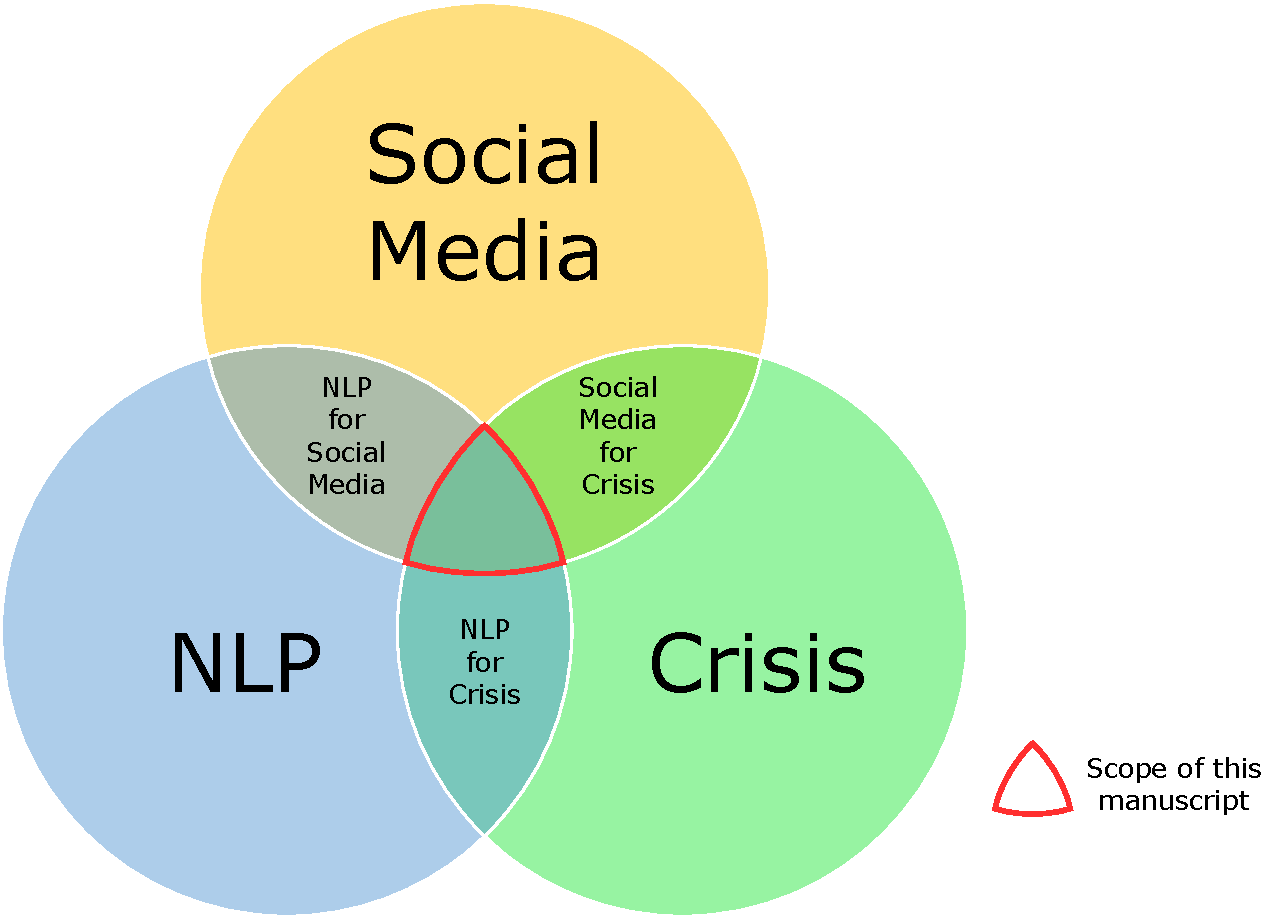
\includegraphics[width=\textwidth]{figures/chap-1/venn-diagram-domains.pdf}
    \caption{Intersection between the domains of Social Media, Crisis Management et Natural Language Processing and the positioning of the research presented in this manuscript.}
    \label{context:venn-diagram-domains}
\end{figure}

\textcite{palenCitizenCommunicationsCrisis2007} highlighted in 2007 the role of information and communication technologies (ICT) in crisis response.
A few years later, social media were considered as an opportunity in crisis management \parencite{viewegMicrobloggingTwoNatural2010}.
This work started the social media branch of crisis informatics \parencite{palenCrisisInformaticsHumancentered2020}.
NLP was then used to automatically retrieve information from the flow of social media data \parencite{vermaNaturalLanguageProcessing2011,carageaClassifyingTextMessages2011}.
This allowed scaling the analysis to the high volume of content that social media have to offer.
Most of the early work was spent in ways to identify crisis-related text messages automatically.
Since then, many efforts have been added to explore other opportunities, such as images.
Variations on different crises, NLP techniques, and features used to represent the data were developed and used.
\textcite{imranUsingAISocial2020} identify several remaining challenges in the domain of social media in crisis informatics:

\begin{itemize}
    \item Crisis event detection: detect the apparition of an event by detecting characteristics messages.
    \item Eyewitness detection: determine whether a direct or indirect eyewitness posts a message.
    \item Situational awareness: identify text messages that contribute to restoring the situational awareness of crisis management organization
    \item Actionable information gathering: a collection of information that facilitates decision-making
    \item Damage assessment: methods to determine the extent of the damage caused.
    \item Crisis communication: tools to facilitate crisis communication to the general public
    \item Understanding public reaction: tools to help understand the general public reactions to an event
    \item Information veracity: evaluation of the relevance of the information collected
\end{itemize}

All these challenges aim at extracting information from social media.
They necessarily involve artificial intelligence to identify at scale the mentioned information.
However, as mentioned earlier, social media data are subjective, fuzzy, and prone to rumors.
At the same time, the outcome of NLP models is never 100\% accurate.
Thus, uncertainty is the norm among the information extracted from social media data.
Also, all this information, once created, need to be stored, managed, and distributed to provide valuable insights.
Thus, the following research question:

\begin{center}
    \fbox{
        \begin{minipage}{0.75\textwidth}
            \centering
            \emph{Primary research question:}

            How to design an information system for crisis response that can automatically manage and deliver actionable information from social media data?
        \end{minipage}
    }
\end{center}

This primary research question is then decomposed into three sub-research questions.

\subsection{Challenges consecutive to the primary research question}
Three consecutive challenges arise.
In order to collect actionable information, the first step is to define what is actionable information in our context.
Hence,

\begin{center}
    \fbox{
        \begin{minipage}{0.75\textwidth}
            \centering
            \emph{Research question 1:}

            What can decision-relevant information from social media be processed automatically?
        \end{minipage}
    }
\end{center}

Using the previous results, i.e., the actionable information for the decision-makers, leads to the question of the automated recovery of this information.
Hence, the second research question:

\begin{center}
    \fbox{
        \begin{minipage}{0.75\textwidth}
            \centering
            \emph{Research question 2:}

            How can the actionable information available on social be automatically retrieved during crisis response?
        \end{minipage}
    }
\end{center}

Finally, obtaining this information allows us to answer the automatic information retrieval part.
The last part is thus interested in the aspects of management and distribution of information.
In particular, how should this system be designed if it uses machine learning models to obtain information?
Leading to the third research question:

\begin{center}
    \fbox{
        \begin{minipage}{0.75\textwidth}
            \centering
            \emph{Research question 3:}

            What are the challenges faced by an information system dedicated to crisis management that embeds machine learning models?
        \end{minipage}
    }
\end{center}

\subsection{Research context}
This chapter has presented three scientific topics whose main research question is at the intersection.
This Ph.D., whose subject is at the border between social sciences and information sciences, has brought together three main academic actors.
These three partners reflect the multidisciplinary approach taken during this Ph.D.

The MACIV project (Management of Citizens and Volunteers: the social media contribution in crises) brought together a variety of actors from different institutions around the issue of the adoption of social media in crisis response.
The project studied the opportunity offered by volunteers in crisis management, emphasizing contributions on social media.
This project, funded by the Agence National de la Recherche (ANR), was composed of both
scientific actors — Télécom ParisTech, IMT Mines Albi and —,
institutional actors — Direction Générale de la Sécurité Civile et de la Gestion des Crises, Préfecture de Police de Paris, Service Départemental d'Incendie et de Secours du Var — and
associatives actors — the VISOV (Volontaires Internationaux en Soutien Opérationel Virtuel) association.
Under the principal supervision of Dr. Caroline Rizza from Telecom Paris, this collaboration was illustrated through three different real-world exercises.
These exercises were an opportunity to meet, observe and exchange with crisis management practitioners in France.
The MACIV project has also seen the completion of two doctoral degrees.
The first one was presented and defended by Robin Batard \parencite{batardIntegrerContributionsCitoyennes2021}.
The second one is currently in front of the reader.
The former was interested in the role played by citizens in response to an event and how they could be integrated into the official organization.
His findings and observations inform this paper, particularly on the contributions related to the social sciences.

This Ph.D. also involved PennState University, through the co-direction of Pr. Andrea Tapia.
Although this project was conducted primarily in France, a year-long visit to the U.S. considerably benefited this work.
This exchange was an occasion to understand the challenges of the research question through the point of view of the social sciences, which informs chapters three and five.
It also created the opportunity to meet several actors of the American emergency services, such as the Charleston County 911 Center and Cincinnati 911 operators, among others.
These meetings provided valuable insights as well as a different perspective on the organization of crisis management.

Finally, this work was mainly conducted in France at IMT Mines Albi under the direction of Pr. Frederick Benaben and supervision of Dr. Aurélie Montarnal.
PennState University provided valuable insights on the social science side of the research topic.
However, this Ph.D. focus is in information sciences.
Chapters four and five reflect the body of work conducted at IMT Mines Albi.
Most importantly, the research topic emerged from a reflection on connecting the R-IO Suite software to social media.
The R-IO Suite software\footnote{https://research-gi.mines-albi.fr/display/RIOSUITE/R-IOSuite+Home} is "a dedicated set of tools to support efficiently inter-organizational collaborations."
The software is articulated around an information model that represents the different concepts handled by the software.
As several scenarios exist in which inter-organizational collaborations can happen, the model is declined in several flavors.
This model related to crisis management is further explained in section \hyperref[sec:crisismetamodel]{3.2.1}.
R-IO Suite is composed of a variety of services that handle different aspects of inter-organizational collaborations.
Its services are visually represented in Figure~\ref{context:rio-services}.

\begin{figure}[htb]
    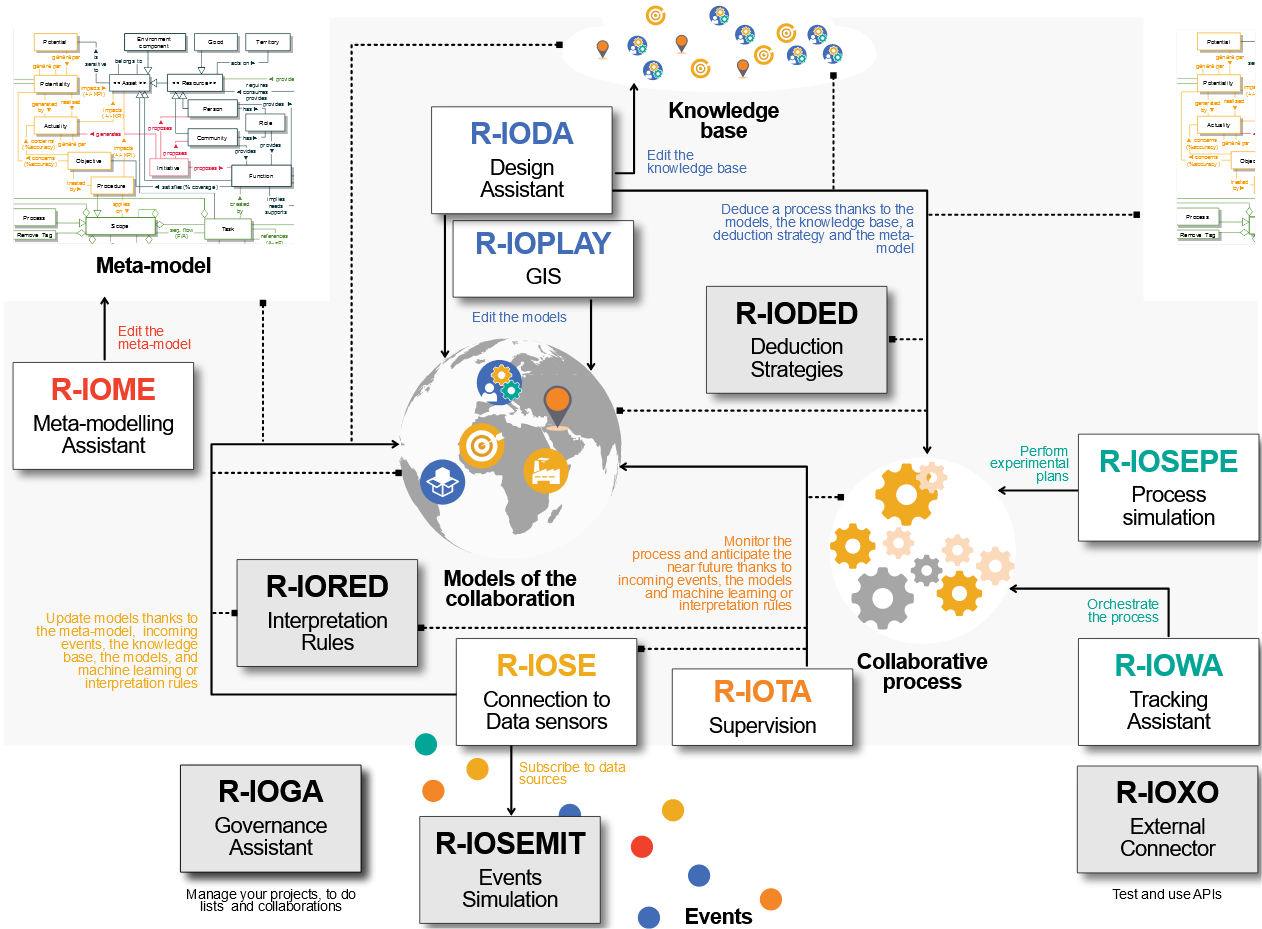
\includegraphics[width=\textwidth,keepaspectratio]{figures/chap-1/rio-services.png}
    \caption{Services that compose R-IO Suite.}
    \label{context:rio-services}
\end{figure}

The main services are:

\begin{itemize}
    \item R-IOPLAY: provides a Common Operational Picture
    \item R-IODED: proposes strategies to address certain aspects of the event
    \item R-IOSE: connects to a variety of data sources
    \item R-IOSEMIT: performs simulations of the outputs of R-IOSE
    \item R-IORED: is in charge of processing the data provided to instantiate the classes of the information model
    \item R-IOME: the editor of the information model
    \item R-IOGA: the main interface of R-IO, manages the different projects and use cases available
\end{itemize}

\section{Structure of the document}
The purpose of this manuscript is to advance the issue of improving situational awareness and collaboration between actors during the response to a crisis event, which was one of the issues identified in the crisis management section.
Thus, adopting the point of view of decision-makers, and in the scope of the information system, the principal research question is:

\emph{How to design an information system for crisis response that can automatically manage and deliver actionable information from social media data?}

The scope and consecutive research questions of the primary one are illustrated in Figure~\ref{context:big-picture}.

\begin{landscape}
    \begin{figure}[htb]
        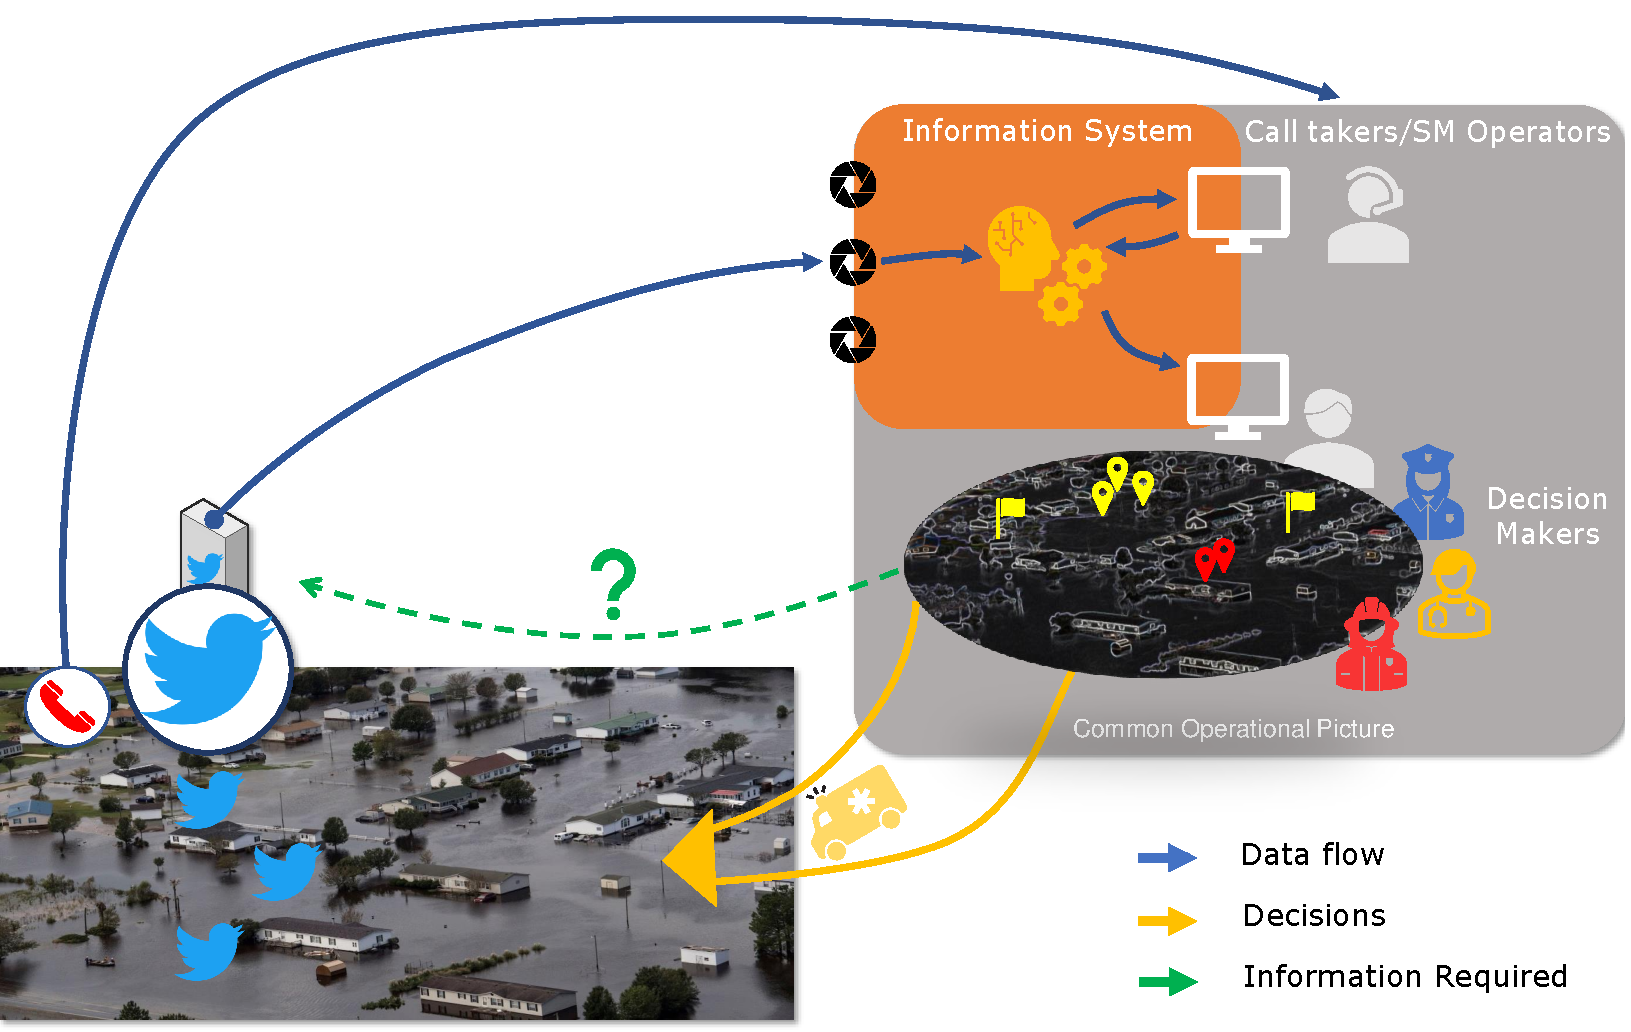
\includegraphics[width=\textwidth,height=\paperheight,keepaspectratio]{figures/chap-1/big-picture.pdf}
        \caption{Big picture of the manuscript.}
        \label{context:big-picture}
    \end{figure}
\end{landscape}

\begin{figure}[htb]
    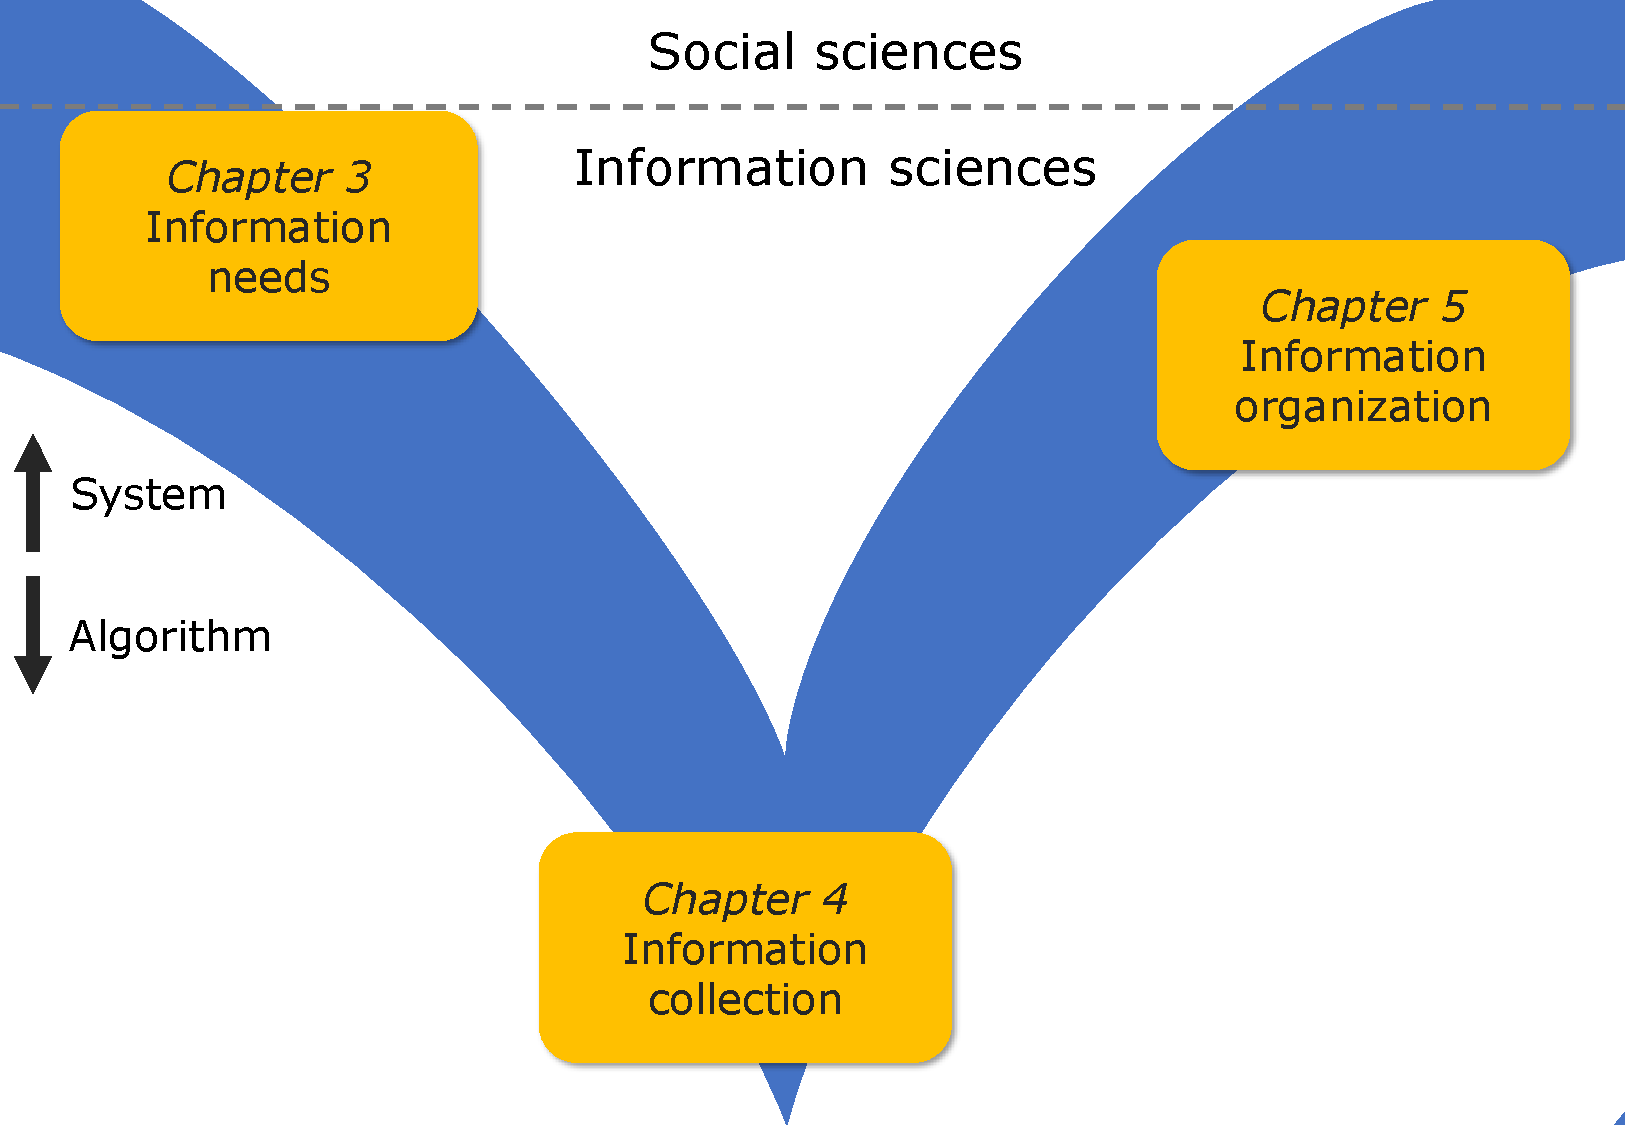
\includegraphics[width=\textwidth]{figures/chap-1/dissertation-plan.pdf}
    \caption{Organization of the different contributions presented in this dissertation.}
    \label{context:plan}
\end{figure}

The following chapter, Chapter 2, is a literature review that explores the scope of each research question.
Chapters 3 to 5 are the contributions associated with each research question.

\begin{itemize}
    \item Chapter 3 narrows the scope of the information system designed by identifying its users and their information needs from an operational point of view.
    \item Chapter 4 describes an algorithm to identify the information needed while maintaining the user in the information extraction process.
    \item Chapter 5 embeds all the previous contributions in software architecture for a crisis information system, allowing to structure and produce further information.
\end{itemize}

The final chapter, chapter 6, provides conclusions and discussions about this work.

%%% Local Variables:
%%% mode: latex
%%% TeX-master: "../ma-these"
%%% End:
